\section{Permutations}
Ladder lotteries and permutations are intricately related to each other. Each $\pi$ has an $OptL\{\pi\}$ such that 
each ladder form $OptL\{\pi\}$ sorts $\pi$. The so called Listing Problem is one of the problems addressed in this thesis.
In brief, this problem is about how to list all $n!$ ladders efficiently. The research for this problem is highly influenced 
by permutation enumeration research. Knuth describes a number of 
permutation enumeration algorithms in The Art of Computer Programming~\cite{A18}. Since this book, many algorithms for 
enumerating $n!$ permutations have been created. During the research for the Listing Problem, twelve of these 
enumeration algorithms were investigated~\cite{A18}\cite{A19}\cite{A21}\cite{A24}\cite{A25}\cite{A26}\cite{A31}\cite{A34}\cite{A35}\cite{A36}\cite{A37}. 
The first is the lexicographic algorithm which orders all $n!$ permutations from smallest to largest. The lexicographic 
algorithm generates each permutation with an amortized time of $O(n^{2}log(n))$~\cite{A21}. The second of which is the 
colexicographic algorithm which orders all $n!$ permutations from largest to smallest. The colexicographic 
algorithm generates each permutation with an amortized time of $O(n^{2}log(n))$~\cite{A19}. The third of which is Zak's 
algorithm which generates all $n!$ permutations by reversing a suffix in one permutation to get to the next 
permutation. The time complexity of Zak's algorithm is amortized time of $O(n^{2})$~\cite{A31}.
The fourth of which is Heap's algorithm which is a decrease and conquer algorithm.  
The time complexity of Heap's algorithm is {\sc CAT}, constant amortized time of $O(1)$ per permutation~\cite{A24}.
The fifth algorithm is the Steinhaus-Johnson-Trotter algorithm which generates $S_{n}$ by performing adjacent swap operations 
on the permutation resulting in the next permutation. Thus, each permutation in $S_{n}$ differs 
from it predecessor by a single swap operation~\cite{A25}. To go From any two successive permutations, 
the time complexity is $O(1)$~\cite{A25}.
The sixth algorithm is the algorithm using star transpositions that always swaps the first element of the permutation 
with some other element. It was discovered by Gideon Ehrlich and is described as Algorithm E in Knuth's book~\cite{A18}.
The seventh algorithm is the derangement ordering in which no two consecutive permutations have any elements 
in the same position. It was first discussed by Savage in~\cite{A35}. 
The eighth algorithm is the Single Track listing algorithm. Each column in the list of permutations 
is a cyclic shift of the first column~\cite{A36}. The computation for each successive permutation 
is CAT~\cite{A36}.
The ninth algorithm is the Single Track Gray Code listing algorithm. The properties of the Single Track 
listing algorithm hold. Furthermore, any two successive permutations differing by at most two transpositions~\cite{A36}.
The tenth listing algorithm is found in Knuth's book. At each step, it either rotates the permutation to the left by one 
or swaps the first two elements~\cite{A37}. The problem as to whether such a listing algorithm exists for all $n$ 
is posed as an open problem in Knuth's book~\cite{A37}. It was solved by Sawada and Williams in their paper 
A Hamiltonian Path for the Sigma-Tau Problem~\cite{A38}.
The eleventh algorithm is Corbett's algorithm which rotates a prefix of the first possible length in 
$n$,$2$,$n-1$,$3$,$n-2$,$4$, etc.~\cite{A34}. 
The twelfth algorithm is Effler and Ruskey's algorithm which lists permutations by groups of $k$ inversions. Their algorithm has 
constant amortized time algorithm for generating permutations of order $n$ with $k$ inversions~\cite{A26} meaning 
the time it takes to generate each permutation is bounded by a constant.
The algorithm is also a \emph{BEST} algorithm (backtracking ensures success at terminals), meaning that when the algorithm backtracks, 
the back-tracking leads to a successful result~\cite{A26}. Please refer to 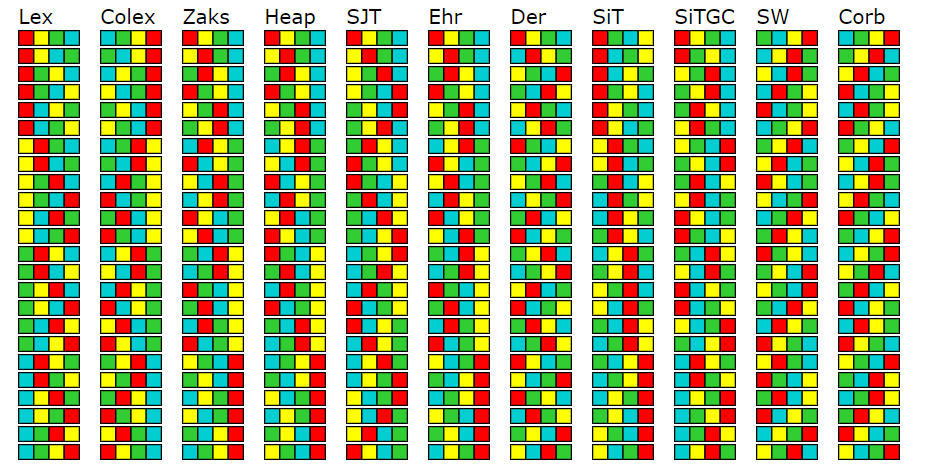
\includegraphics{11perms} to see eleven of the twelve 
listings of permutations for $n=4$.\par 
In Chapter 1, it was already stated that Algorithms~\cite{A25}\cite{A26} were the most conducive for The Listing Problem. 
These are the Steinhaus-Johnson-Trotter and Effler-Ruskey algorithms respectively. Each of these two algorithms are 
advantageous for differing reasons. The reason that the SJT algorithm is beneficial is because it generates each 
permutation in $O(1)$ per ladder; thus making it extremely efficient. In Chapter 3, the SJT 
algorithm is modified to create ladders instead of permutations while still maintaining the same efficiency.
The reason that the Effler-Ruskey algorithm 
is beneficial is because it has a nice ordering property in which the permutations are listed by the number of inversions.
The algorithm is still fairly efficient due to it being BEST and CAT. In Chapter 3, the Effler-Ruskey algorithm 
is modified to create ladders by $k$ bars, though in doing so it loses some of the efficiency of the permutation listing algorithm.
When the SJT and Effler-Ruskey algorithms are modified for ladders, it is always the root ladder from each 
$OptL\{\pi\}$ which is listed by each of the algorithms. This allows for simplicity when 
listing all $n!$ ladders. It is for these aforementioned reasons that the SJT algorithm and Effler-Ruskey 
algorithms were chosen to solve the Canonical Listing Problem in Chapter 3.



